\documentclass{optica-article}

\journal{opticajournal}

\articletype{Research Article}

\usepackage{lineno}
\linenumbers

\usepackage{amsmath}
\usepackage{physics}
\usepackage{siunitx}
\AtBeginDocument{\RenewCommandCopy\qty\SI}
\usepackage{booktabs}
\usepackage{subcaption}

\begin{document}

\title{Ultrafast Burst-Driven Collective Nonlinear Absorption for Enhanced Photoacoustic Signal Generation}

\author{Burak Arayit\authormark{1,*}}

\address{\authormark{1}Department, Institution, City, Country}

\email{\authormark{*}email@institution.edu}

\begin{abstract*}
Ultrafast burst-mode excitation, consisting of closely spaced sequences of femtosecond pulses, enables regimes of light--matter interaction that are not accessible with isolated pulses. We show that such bursts can induce a collective absorption process in which early pulses generate free carriers through two-photon excitation, increasing the effective absorption experienced by subsequent pulses. This produces a transition from purely nonlinear absorption to a combined nonlinear--linear regime governed by Auger-limited carrier accumulation. We develop an analytical model coupling two-photon carrier generation with Auger recombination, yielding a piecewise-exact solution for the carrier dynamics and a closed-form expression for the burst enhancement factor. The enhancement separates into a direct intensity-scaling contribution and a free-carrier contribution characterized by a single dimensionless parameter---the steady-state ratio of free-carrier to two-photon absorption. We illustrate the implications for photoacoustic signal generation, where the enhanced energy deposition enables efficient localized heating under conditions where conventional excitation is limited.
\end{abstract*}

\section{Introduction}

Deep optical resolution plays a crucial role in biological sciences, and many imaging modalities have been developed to achieve high lateral resolution at deeper sections of biological tissue \cite{Yoon-2020}. High resolution microscopy for sub mm range is clinically significant for the determination of staging of melanoma tumors, monitoring drug delivery and imaging of tumor cores where drug resistance develops \cite{balch2009, aguirre2025,vakoc2009,minchinton2006}. However, there is a fundamental trade-off between high resolution and imaging depth due to optical scattering in complex media \cite{Yoon-2020}. Modalities such as confocal microscopy, stimulated emission depletion (STED), photoactivated localization microscopy (PALM), and super-resolution optical fluctuation imaging (SOFI) can achieve subcellular lateral resolution ($<1~\mu$m), but their imaging depth is limited to approximately 100--200 $\mu$m \cite{Yoon-2020}. Optical coherence tomography (OCT), optical coherence microscopy (OCM), and multiphoton microscopy (MPM) can reach depths on the order of 1 mm, but their lateral resolution degrades with depth \cite{Yoon-2020, Helmchen-2005}. Near-infrared (NIR) light scatters less in biological tissue compared to visible light; thus, it can penetrate deeper without undergoing scattering events \cite{Bashkatov-2005}.

Despite NIR light penetrating deeper into tissue, multiphoton microscopy, specifically two-photon microscopy, cannot image beyond 1 mm due to background fluorescence \cite{Helmchen-2005}. Upon two-photon (or three-photon) absorption, the emitted fluorescence photons have twice the frequency of the incident photons, placing them in the visible range \cite{Denk-1990}. During collection, visible photons undergo significantly higher scattering \cite{kobat-2009}. Thus, even though NIR light can reach deeper sections of biological tissue, collection of the fluorescence photons remains a limiting factor for MPM \cite{kobat-2009}. Theer demonstrated that the two-photon microscopy depth limitation arises from background fluorescence, which is caused by scattered photons outside the focused region along the beam path \cite{theer-2006}. While using longer excitation wavelengths can improve penetration depth, fluorescence-based detection remains inherently limited by collection efficiency---motivating alternative detection mechanisms \cite{kobat-2009}.

The fluorescence collection problem can be addressed by employing photoacoustic detection \cite{Xu-2006}. Unlike fluorescence, the generated acoustic waves propagate with minimal scattering, enabling signal detection from deeper regions \cite{Maslov-2008}. Multiphoton absorption can provide optical contrast independent of linear absorption properties, with signal scaling nonlinearly with intensity and providing inherent localization to the focal volume \cite{Helmchen-2005}. To resolve this problem, various contrast agents can be employed to increase contrast in the deeper section of the tissue, specifically tuned to have multiphoton absorption at NIR. Notably, exogenous contrast agents are widely used for clinical applications such as cancer imaging \cite{Vahrmeijer2013}, and the NIR window allows usage of many bio-compatible organic and inorganic compounds, offering tunability for certain applications \cite{shaw2022two}. As an example, silicon nanoparticles are widely used in medicine and biology as a contrast agent for theranostic and diagnostic purposes, such as imaging and therapy for cancer, biosensing, and cell imaging \cite{ofarrell2006,peng2014,arap2013, mochizuki2021}. Moreover, their semiconductor nature allows creation of free carriers through nonlinear excitation, where it increases absorption capability of the particle \cite{trinh2012, boggess1986}.

Multiphoton photoacoustic imaging is highly desirable due to its high optical resolution combined with long-range ultrasound detection capability \cite{lai2014nonlinear}. Several attempts have been made in the last decade to realize multiphoton photoacoustics; however, these attempts have been largely unsuccessful. Previous studies demonstrated that single femtosecond pulses deliver a low amount of energy compared to conventional nanosecond systems. Even though femtosecond pulses can achieve high optical intensity, they are incapable of producing sufficient acoustic pressure due to the low pulse energy. Since the photoacoustic signal is directly proportional to the absorbed energy density, the multiphoton-induced signal remains too weak for practical imaging \cite{Xu-2006}. While maintaining pulse intensity below the ablation threshold and total power within thermal damage limits, conventional ultrafast lasers cannot deliver sufficient energy for photoacoustic signal generation \cite{boyd-2008}.

A method combining high energy delivery with nonlinear excitation could enable practical multiphoton photoacoustic imaging. In this work, we propose a method that utilizes an ultrafast GHz-burst-mode laser to generate a strong photoacoustic signal induced by multiphoton absorption \cite{kerse2016}. Unlike conventional femtosecond systems limited by single-pulse energy, burst mode accumulates energy from multiple pulses while each individual pulse remains below the ablation threshold, enabling high total energy delivery without sacrificing the high peak intensity required for nonlinear absorption. GHz-burst mode delivers hundreds of femtosecond pulses within a nanosecond time window, ensuring that the total energy delivery time falls within the stress confinement time, $\tau_{\text{st}}$, while also satisfying thermal confinement. All pulses contribute to heating of the target tissue, which in turn generates the photoacoustic wave. The resulting photoacoustic pressure $P$ is proportional to the heating function $H$ ($P \propto H$) \cite{wang-2007}. Since the photoacoustic wave amplitude is directly related to the amount of heating, the signal can be increased by adding more pulses within the $\tau_{\text{st}}$ time window. When combined with silicon nanoparticles, further amplification of the resulting photoacoustic signal with consecutive pulsing can be enabled by burst-mode operation. This signal enhancement could enable practical multiphoton photoacoustic imaging.

\section{Theory}

\subsection{Photoacoustic generation}

High-intensity modulated light causes a rapid heat rise, which results in subsequent rapid expansion and hence creates a photoacoustic wave. Two primary time scales govern this process: the thermal confinement time $\tau_{\text{th}} = d_c^2/4\kappa_{\text{th}}$, over which deposited energy dissipates via thermal diffusion, and the stress confinement time $\tau_{\text{st}} = d_c/v_s$, over which mechanical stress relaxes. Here, $d_c$ is defined as the characteristic dimension and represents the dimensions of the heated region, $v_s$ is the speed of sound, and $\kappa_{\text{th}}$ is the thermal diffusivity in the medium \cite{xu2006photoacoustic}. When both thermal confinement ($\tau \ll \tau_{\text{th}}$) and stress confinement ($\tau \ll \tau_{\text{st}}$) conditions are met, the initial rise in pressure induced by optical excitation can be calculated by the following formula \cite{wang-2007}:
\begin{equation}
p_0 = \Gamma \cdot H
\label{eq:general_pa}
\end{equation}
where $\Gamma$ is the Gr\"uneisen parameter, which reflects the photoacoustic characteristic of the target, defined as $\Gamma = \alpha v_s^2/C_p$, where $\alpha$ is the isobaric volume expansion coefficient in K$^{-1}$, $C_p$ is the specific heat capacity in J/(K$\cdot$kg).

\subsection{Free carrier effects}

When a strong laser field, up to $\text{TW}/\text{cm}^{2}$ \cite{keller2003recent-2a2}, produced by an ultrafast burst-mode laser interacts with a semiconductor, early ultrafast pulses within the burst can generate free carriers by exciting electrons across the band gap via multiphoton absorption \cite{schroder1978}. Free carriers are generated via two-photon absorption as follows, assuming $2\hbar\omega>E_g$ where $E_g$ is the band-gap energy of the semiconductor:
\begin{equation}
\frac{dN_\text{fc}}{dt} = \frac{\beta}{2\hbar\omega}\,I^2(t) - \gamma\,N_\text{fc}^3
\label{eq:n_fc}
\end{equation}
where $N_\text{fc}$ is the free-carrier density, $\beta$ is the two-photon absorption coefficient, and $\gamma$ is the Auger recombination constant \cite{othonos1998,driel1986}. The first term describes carrier generation through nonlinear absorption, while the second term accounts for Auger recombination which is the dominant mechanism at high carrier densities \cite{driel1986}. The pulse train of Gaussian burst of $N$ pulses can be analytically expressed as:
\begin{equation}
I(t) = I_p \sum_{n=0}^{N-1} \exp\!\left[-\frac{4\ln 2}{\tau_\text{p}^2}\,(t - n\,\tau_\text{r})^2\right]
\label{eq:pulse_train}
\end{equation}
where $I_p$ is the peak intensity, $\tau_\text{p}$ is the pulse FWHM, and $\tau_\text{r}$ is the inter-pulse spacing. Since $\tau_\text{p} \ll \tau_\text{r}$, the pulses do not overlap and recombination is negligible during each pulse. Integrating the generation term over a single Gaussian pulse gives the per-pulse carrier increment:
\begin{equation}
\Delta N_\text{fc} = \frac{\beta\,I_p^2\,\tau_\text{p}}{2\hbar\omega}\,\sqrt{\frac{\pi}{8\ln 2}}
\label{eq:deltaN}
\end{equation}
Between pulses, only Auger recombination acts, yielding the recurrence relation which gives the carrier density just before the next pulse:
\begin{equation}
N_{n+1} = \frac{N_n + \Delta N_\text{fc}}{\sqrt{1 + 2\gamma\left(N_n + \Delta N_\text{fc}\right)^2 \tau_\text{r}}}
\label{eq:recurrence}
\end{equation}
with $N_0 = 0$. The accumulated carriers absorb linearly with free-carrier absorption (FCA) cross section $\sigma_\text{fc}$ \cite{boggess1986}, contributing to the total heating alongside direct TPA.

\subsection{Burst-mode enhancement}

Generating a photoacoustic signal via nonlinear excitation requires high optical intensity levels. While decreasing the pulse duration is the most direct method to increase light intensity, this consequently reduces the energy per pulse, preventing the generation of desired photoacoustic signal levels. To overcome this trade-off, we propose employing burst-mode, high-repetition-rate ultrafast lasers. This approach packages multiple high-intensity ultrafast pulses into a single envelope. By ensuring the total burst duration ($\tau_\text{burst}$) remains within the stress confinement time ($\tau_\text{burst} \ll \tau_{\text{st}}$), a high total energy can be delivered, leading to the generation of high-amplitude photoacoustic pressure.

To compare these scenarios fairly, both must operate within safe intensity limits for biological tissue. The critical intensity for tissue damage scales with pulse duration as $I_c \propto \tau_p^{-\omega}$, where the exponent $\omega$ depends on the dominant damage mechanism \cite{Stuart1996LaserBreakdown, Vogel2007}. For the nanosecond pulse regime, thermal diffusion limits damage ($\omega \approx 0.5$), while in the ultrafast regime, multiphoton ionization dominates and $\omega$ becomes $\omega \approx 0.7$--0.8 \cite{Giguere2007, Sun2007CornealAblation}. Assuming both scenarios operate at equivalent safety margins:
\begin{equation}
I_p = I_0 \left(\frac{\tau_0}{\tau_p}\right)^\omega
\label{eq:intensity_scaling}
\end{equation}
For further calculations, we assume $\omega = 0.75$ \cite{Giguere2007}.

To quantify the enhancement provided by burst-mode operation, we define the enhancement factor $\varepsilon = H_{\text{burst}}/H_{\text{ns}}$, where $H_{\text{ns}} = \beta\,I_0^2\,\tau_0$ is the heating from a single nanosecond reference pulse. The total burst heating separates into TPA and FCA contributions:
\begin{equation}
H_{\text{burst}} = N\,\beta\,I_p^2\,\tau_\text{p}\,\sqrt{\frac{\pi}{8\ln 2}} + \sigma_\text{fc}\,I_p\,\tau_\text{p}\,\sqrt{\frac{\pi}{4\ln 2}} \sum_{n=0}^{N-1} N_n
\label{eq:heat_fca_burst}
\end{equation}
where the first term is direct TPA (identical for each pulse) and the second is FCA, which depends on the accumulated carrier density $N_n$ given by Eq.~(\ref{eq:recurrence}). The enhancement likewise separates as $\varepsilon = \varepsilon_\text{TPA} + \varepsilon_\text{FCA}$. Using the intensity scaling from Eq.~(\ref{eq:intensity_scaling}) with $\omega = 0.75$, the TPA enhancement reduces to:
\begin{equation}
\varepsilon_\text{TPA} = N\,\sqrt{\frac{\tau_0}{\tau_p}}\,\sqrt{\frac{\pi}{8\ln 2}}
\label{eq:enhancement_tpa}
\end{equation}
Once the carrier density reaches steady state, where generation and recombination balance ($N_{n+1} = N_n \equiv N_\text{ss}$), the total enhancement factors as:
\begin{equation}
\varepsilon = \varepsilon_\text{TPA}\!\left(1 + \frac{\sqrt{2}\;\sigma_\text{fc}\,N_\text{ss}}{\beta\,I_p}\right)
\label{eq:enhancement_fca}
\end{equation}
The dimensionless ratio $\sigma_\text{fc}\,N_\text{ss}/(\beta\,I_p)$ is the steady-state FCA-to-TPA absorption ratio, quantifying the additional contribution of free-carrier effects beyond direct TPA enhancement.

% ======================================================================
% REWRITE PLAN — Section 3: Analytical Results (replaces Simulation study)
% ======================================================================
%
% OPENING PARAGRAPH:
% To evaluate the enhancement framework derived in Section 2, we apply the
% model to crystalline silicon nanoparticles (c-SiNP) as a representative
% nonlinear contrast agent. Silicon nanoparticles are widely used in
% biomedical applications including biosensing, cell imaging, and cancer
% diagnostics [ofarrell2006, peng2014, mochizuki2021]. Their semiconductor
% nature enables free-carrier generation through multiphoton excitation,
% making them a suitable platform to demonstrate the collective absorption
% mechanism. For particle dimensions exceeding the Bohr exciton radius of
% silicon (~14 nm), bulk optical properties can be applied [brus1984]; we
% therefore adopt the TPA coefficient and FCA cross section measured for
% bulk crystalline silicon by Boggess et al. [boggess1986]. The parameters
% used are summarized in Table 1.
%
% TABLE 1 UPDATE:
% - Keep optical + material rows
% - Drop acoustic rows (grid spacing, sensor elements, SNR)
% - Remove or update target radius (100-400 nm range)
% - Remove mu_a_target = 1.0 (negligible at 1064 nm, Bronstrup 2010)
% - Gruneisen: decide — keep Gamma_tissue = 0.12 or note Gamma_SiNP ~ 0.8 (Omar 2009)?
%
% 3.1 EXCITATION SCENARIOS (keep most of current 3.4):
% Burst duration tau_b = 1 ns, individual pulse tau_p = 100 fs.
% Intra-burst pulse count N = 100, 500, 1000.
% Focal fluence F_p = 0.1 J/cm^2 (5% of ablation threshold, Giguere2007).
% Intensity scaling gives F_0 = 1.0 J/cm^2 for ns reference.
% Focal intensities: I_p = 1 TW/cm^2, I_0 = 1 GW/cm^2.
%
% 3.2 PULSE-BY-PULSE CARRIER ACCUMULATION (Fig 1):
% Show H_k increasing linearly with pulse number as free carriers
% accumulate. By pulse k=100, FCA exceeds TPA baseline by >10x.
% N_c ~ 3 for Si params — FCA dominates after only a few pulses.
% This illustrates the collective nature: each pulse modifies the
% material state for subsequent pulses.
%
% 3.3 ENERGY DEPOSITION SCALING (Fig 2):
% Total deposited energy vs N. TPA scales as N, FCA scales as N^2.
% FCA dominates beyond N_c ~ 3. Total burst heating exceeds ns
% reference by several orders of magnitude at N=1000. The transition
% from linear to quadratic scaling is the signature of the collective
% absorption regime.
%
% 3.4 ENHANCEMENT FACTOR (Fig 3):
% Enhancement epsilon vs N for three pulse durations (50, 100, 500 fs).
% Shorter pulses yield higher enhancement via (tau_0/tau_p)^0.5.
% For tau_p = 100 fs and N = 1000, enhancement exceeds 10^7.
%
% 3.5 PARAMETER SPACE (Fig 4):
% Contour map of epsilon in (N, tau_p) space. N_c boundary separates
% TPA-dominated from FCA-dominated regime. Enhancements of 10^5--10^9
% accessible across broad experimentally realizable parameters.
%
% ======================================================================

\section{Simulation study}

To validate the theoretical enhancement predictions derived in Section 2 and demonstrate their practical applicability, a simulation study was conducted using realistic biological imaging parameters. To test this hypothesis under controlled conditions, we employed silicon nanoparticles (SiNP) as a nonlinear contrast agent. For the acoustic propagation simulations, we use the k-Wave toolbox for MATLAB, which solves the acoustic wave equations using a k-space pseudo-spectral method, enabling efficient and accurate simulation of photoacoustic wave propagation in homogeneous media \cite{Treeby2010kWave}.

\begin{table}[htbp]
  \centering
  \caption{System parameters used in analytical calculations.}
  \label{tab:params}
  \small
  \begin{tabular}{@{}llS[table-format=1.2e2]l@{}}
  \toprule
  Parameter & Symbol & {Value} & Unit \\
  \midrule
  Wavelength              & $\lambda$       & 1064    & nm \\
  Numerical aperture      & NA              & 0.50    & -- \\
  Refractive index        & $n$             & 1.33    & -- \\
  FS pulse duration       & $\tau_p$        & 100     & fs \\
  FS focal fluence        & $F_p$           & 0.1     & \si{J/cm^2} \\
  Burst window            & $\tau_{\mathrm{burst}}$ & 1 & ns \\
  NS pulse duration       & $\tau_0$        & 1       & ns \\
  NS focal fluence        & $F_0$           & 1.0     & \si{J/cm^2} \\
  \midrule
  Absorption coeff.\ (tissue) & $\mu_a$     & 0.05    & \si{mm^{-1}} \\
  Scattering coeff.\ (tissue) & $\mu_s$     & 5.6     & \si{mm^{-1}} \\
  Gr\"uneisen parameter   & $\Gamma$        & 0.12    & -- \\
  \midrule
  TPA coefficient (c-Si)  & $\beta$         & 1.5e-11 & \si{m/W} \\
  FCA cross section       & $\sigma_{\mathrm{fc}}$ & 5e-22 & \si{m^2} \\
  \bottomrule
  \end{tabular}
  \par\vspace{2pt}
  {\footnotesize Tissue: native grey matter at 1100\,nm \cite{yaroslavsky2002}; c-Si properties at 1064\,nm \cite{boggess1986}.}
\end{table}

\subsection{Medium and contrast agent}

To establish a realistic medium configuration, the surrounding medium properties were chosen as biological tissue, with optical properties taken from experimentally reported native brain grey matter absorption and scattering data at 1100~nm \cite{yaroslavsky2002}. The absorption coefficient of native brain grey matter is $\mu_a = 0.05\,\mathrm{mm}^{-1}$, and scattering $\mu_s = 5.6\,\mathrm{mm}^{-1}$. The mean free path $l_t$ is defined as $l_t = 1/\mu_s$, where $g = 0.92$ is the anisotropy coefficient, giving $l_t \approx 0.18$~mm for our configuration. We use $\mu_t = \mu_a + \mu_s$ as the attenuation coefficient since we count ballistic photons reaching the target.

The target is selected as silicon nanoparticles (SiNP), which are a common contrast agent in nonlinear imaging applications with well-defined optical properties and the capability to produce free carriers \cite{boggess1986, trinh2012}. SiNPs have $\beta = 1.5$~\si{cm/GW} and $\sigma_\text{fca} = 5\times10^{-18}$~\si{cm^2} \cite{boggess1986}.

\subsection{Optical model}

The initial pressure distribution $p_0(\mathbf{r})$ was calculated by modeling the optical excitation and energy deposition within the heterogeneous medium. Our model accounts for realistic beam propagation effects, including absorption and scattering. The excitation laser beam was modeled as a Gaussian profile spatially and focused to the target at varying depths starting from 100~\si{\micro m} to 3~\si{mm} with 500~\si{\micro m} increments. In nonlinear deep tissue imaging applications, the sweet spot for NA is 0.6--0.8, which creates a tighter spot size and achieves better lateral and axial resolution \cite{crosignani2012deep-8f3}. We modeled focusing with a lens having a long working distance and a high numerical aperture NA~$= 0.50$, with $\omega_0 = 0.68$~\si{\micro m} for $\lambda = 1064$~\si{nm}. Light propagation through the medium was simulated using a layer-by-layer approach, where at each depth $z$, the Gaussian beam waist $\omega(z)$ was calculated using standard Gaussian formalism:
\begin{equation}
w(z) = w_0 \sqrt{1 + \left(\frac{z - z_{\text{focus}}}{z_R}\right)^2}
\end{equation}
This approach allows focusing at depth $z_\text{target}$ where $\omega(z_\text{target}) = \omega_0$ ensures tight focusing at the target location. Input peak surface intensity was calculated with input fluence and pulse duration, with the approximation $I \approx F \cdot \tau$. Using the calculated beam waist $\omega(z)$, the intensity map at each depth is:
\begin{equation}
I(y, z) = I_{\text{peak}}(z) \cdot e^{-2y^2 / w(z)^2}
\end{equation}
Including Beer--Lambert attenuation through propagation:
\begin{equation}
\frac{dI}{dz} = -\mu_t(x,y) \cdot I
\label{eq:beam_propagation}
\end{equation}
We used the linear part of the Beer--Lambert law with Taylor series expansion for sufficiently small step size $\Delta z$:
\begin{equation}
I_{\text{peak}}(z + \Delta z) = I_{\text{peak}}(z) \cdot (1 - \mu_t \Delta z)
\end{equation}
where $\mu_t$ is the attenuation coefficient for the surrounding medium. Attenuation due to nonlinear absorption is negligible because the surrounding medium is water-dominated, and water has low linear absorption near 532~nm, which corresponds to two-photon absorption at 1064~nm \cite{litjens1999visible-7ef}. Moreover, since the beam is tightly focused on the target, the Rayleigh range $z_R = 1.8$~\si{\micro m} is short, so we can ignore the $I^2$ term in the attenuation. After intensity is mapped at each location, the generated heat at each cell can be calculated via Eq.~(\ref{eq:heat_fca_burst}) for burst scenarios and Eq.~(\ref{eq:energy_per_pulse}) for the single nanosecond pulse.

The initial pressure distribution was then obtained via the Gr\"uneisen relation, valid under conditions of thermal and stress confinement:
\begin{equation}
p_0(x,y) = \Gamma \cdot H(x,y)
\label{eq:gruneisen}
\end{equation}
where $\Gamma = 0.12$ is the Gr\"uneisen parameter for soft tissue.

\subsection{Excitation scenarios}

Twenty-five excitation scenarios were simulated to demonstrate enhancement through the GHz-PAM modality and compare different cases. To make Eq.~(\ref{eq:pressure_mpa}) valid, the burst duration was set to $\tau_b = \tau_\text{ns} = 1$~\si{ns}; however, $\tau_\text{stress} \approx 0.9$~\si{ns} for $\omega_0 = 0.68$~\si{\micro m} spot size and the nanosecond pulse is barely outside the stress confinement region. Individual femtosecond pulses have $\tau_\text{fs} = 100$~\si{fs}, which satisfies the stress confinement condition. To calculate the delivered heat by the burst, we assume $Q_\text{burst} = N \cdot Q_\text{individual}$, valid since all pulses are delivered within the stress confinement time. The intra-burst repetition rate was varied by keeping $\tau_b$ constant at 100, 500, and 1000~GHz, corresponding to $N = 100$, 500, 1000 pulses within the burst duration.

Fluence for the single femtosecond pulse, $F_p = 0.1$~\si{J/cm^2}, was set to deliver 5\% of the maximum intensity without passing the ablation threshold for human tissue \cite{Giguere2007}. Using Eq.~(\ref{eq:intensity_scaling}), fluence for a single nanosecond pulse is calculated approximately as $F_0 = 1$~\si{J/cm^2}. For given pulse durations, femtosecond pulses have energy $E_{p,\text{fs}} = 0.72$~\si{nJ} and the nanosecond pulse has $E_{p,\text{ns}} = 7.2$~\si{nJ}. Similarly, the femtosecond pulse reaches the focal intensity $I_p = 1$~\si{TW/cm^2} while the nanosecond pulse produces $I_0 = 1$~\si{GW/cm^2}.

\section{Results}

Results of the simulations are presented in Figs.~\ref{fig:1}--\ref{fig:5}.

\begin{figure}[htbp]
    \centering
    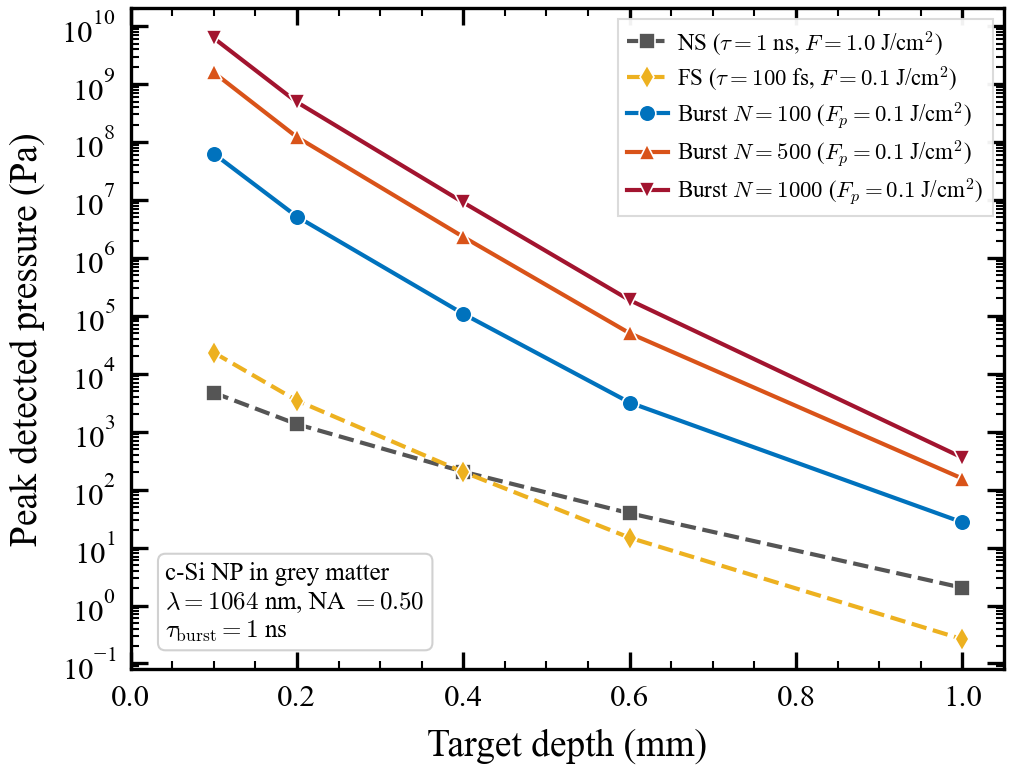
\includegraphics[width=\linewidth]{figures/fig1_peak_pressure_vs_depth.png}
    \caption{Peak detected photoacoustic pressure as a function of target depth for five excitation scenarios.}
    \label{fig:1}
\end{figure}

\begin{figure}[htbp]
    \centering
    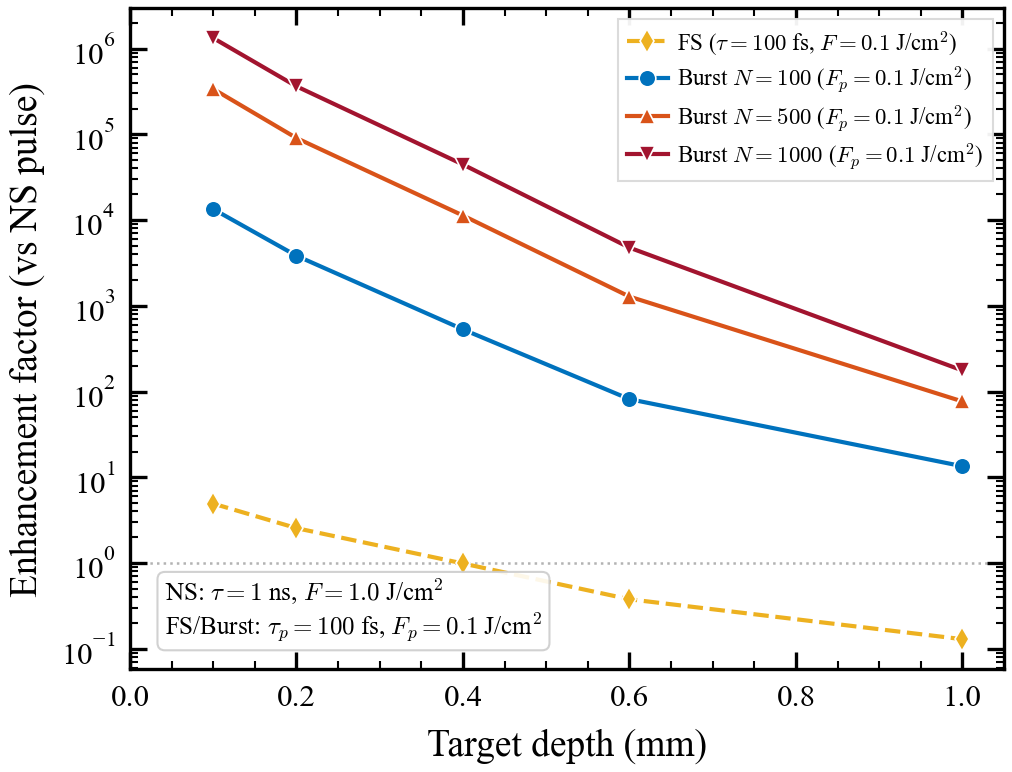
\includegraphics[width=\linewidth]{figures/fig2_enhancement_vs_depth.png}
    \caption{Enhancement factor of each excitation scenario relative to the nanosecond reference pulse as a function of depth.}
    \label{fig:2}
\end{figure}

\begin{figure}[htbp]
    \centering
    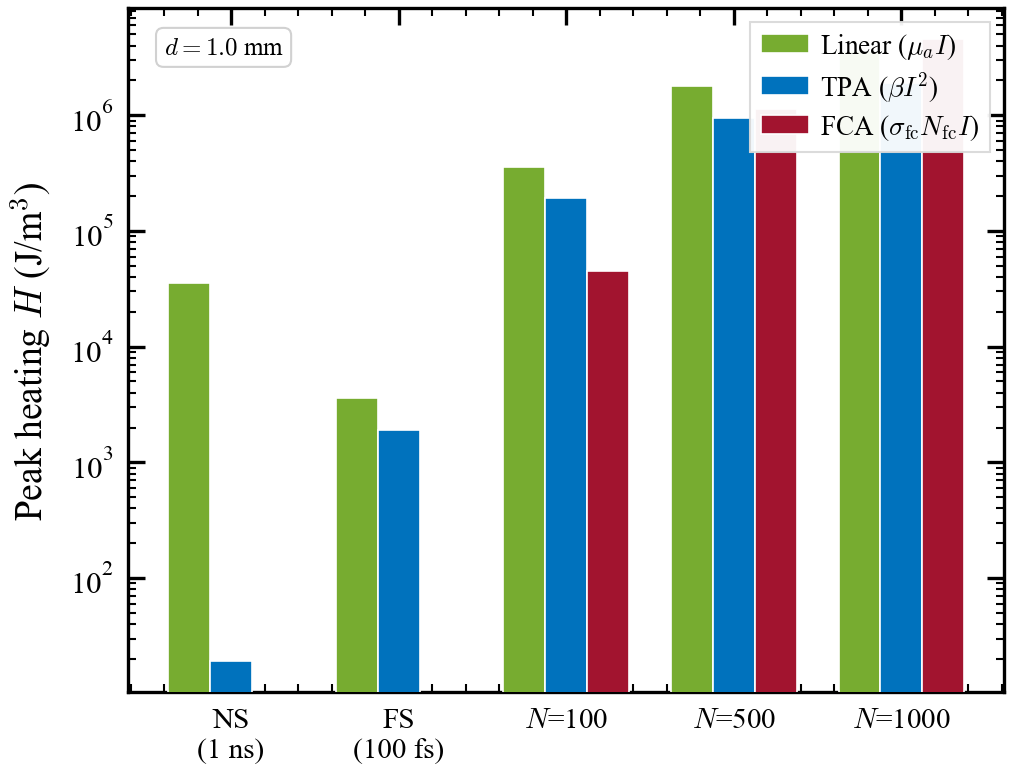
\includegraphics[width=\linewidth]{figures/fig3_heat_breakdown_1.0mm.png}
    \caption{Comparison of linear, TPA, and FCA contributions to peak heating at the focal volume for each excitation scenario at a fixed depth.}
    \label{fig:3}
\end{figure}

\begin{figure}[htbp]
    \centering
    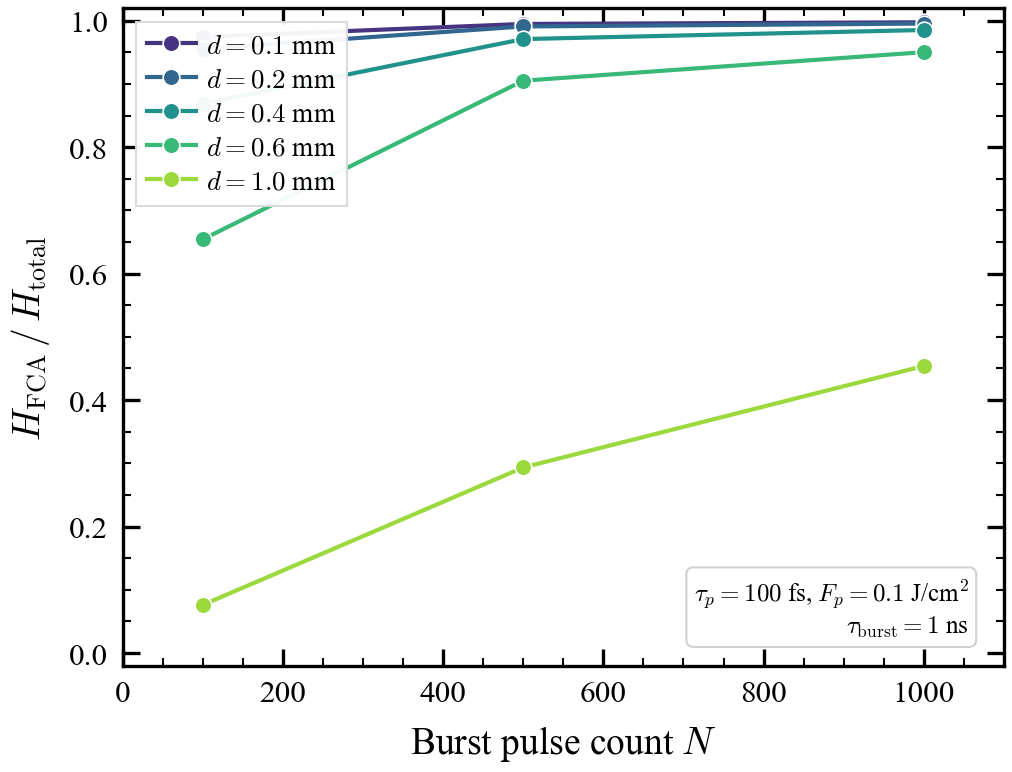
\includegraphics[width=\linewidth]{figures/fig4_fca_fraction_vs_N.png}
    \caption{Fraction of total heating attributed to FCA as a function of burst pulse count for different target depths.}
    \label{fig:4}
\end{figure}

\begin{figure}[htbp]
    \centering
    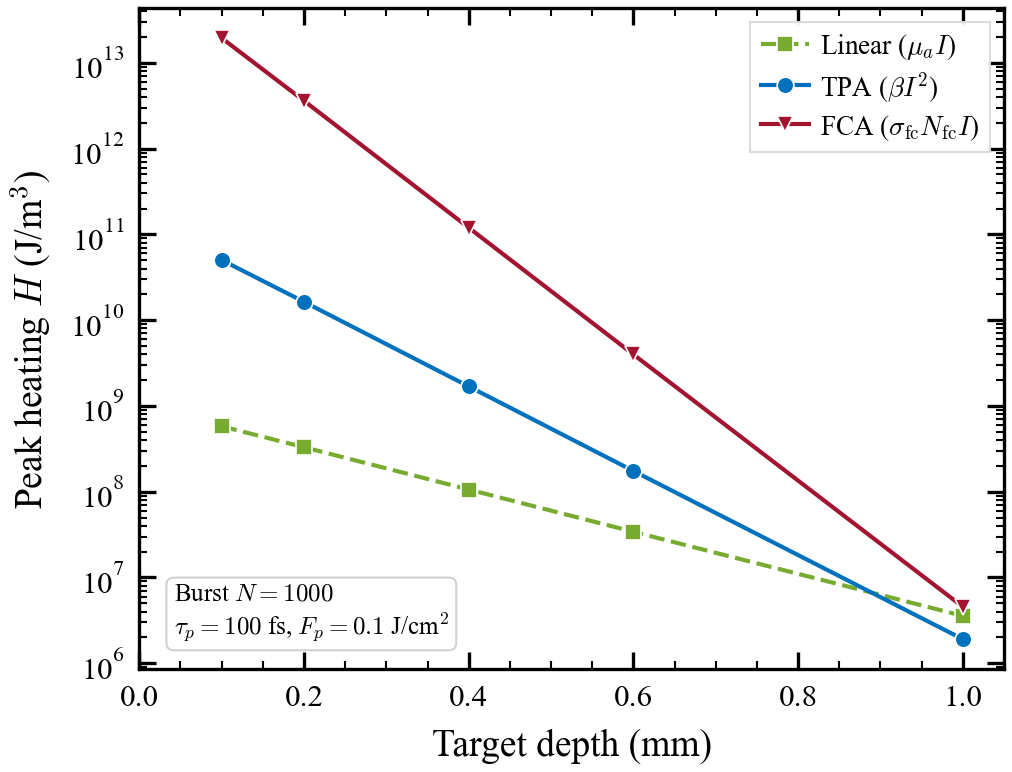
\includegraphics[width=\linewidth]{figures/fig5_heat_vs_depth_N1000.png}
    \caption{Depth dependence of peak linear, TPA, and FCA heating contributions for the $N = 1000$ burst configuration.}
    \label{fig:5}
\end{figure}

\section{Discussion}

To create high intensities to induce multiphoton absorption effects, narrow spot-size configurations are necessary. Reducing the spot size results in a smaller light--material interaction surface, which determines $d_c$. As demonstrated in the simulation, the stress confinement condition is challenging to achieve for nonlinear photoacoustic imaging applications.

Lower pulse energies increase the feasibility for future imaging applications, allowing higher repetition rates without entering the thermal damage regime, which is determined around 2.5~mW for nonlinear imaging applications \cite{hopt-2001}. However, at relatively high intensities produced by ultrafast lasers ($\text{GW}/\text{cm}^{2}$), optical breakdown occurs as plasma starts to form due to avalanche ionization \cite{boyd-2008}. This process is named \textit{plasma-induced ablation} and results in rapid vaporization of the incident surface \cite{Niemz2019}. Since the proposed application is designed to operate at high intensities close to the ablation-threshold regime, pulse energies need to be set carefully.

Laser-induced optical breakdown exhibits different pulse-scaling behavior for different pulse regimes. In the nanosecond regime where $\tau > 500$~ps, the fluence threshold shows an $F_\text{th} \propto \tau^{0.5}$ relationship. In the picosecond regime, $1~\text{ps} < \tau < 500~\text{ps}$, deviations from the $\tau^{0.5}$ curve begin and the curve presents a relationship $\omega = 0.6$--0.8 depending on the material or tissue. The ablation threshold starts to decrease slowly in this regime, as shown experimentally for biological tissues in many studies \cite{Stuart1996LaserBreakdown, Giguere2007, Sun2007CornealAblation}. After entering the $\tau < 1$~ps regime, the relationship enters a plateau regime where $F_\text{th}$ remains constant due to negligible thermal and collision losses during the ultrashort interaction time \cite{loesel1996laserinduced-a8e}.

\begin{figure}[htbp]
    \centering
    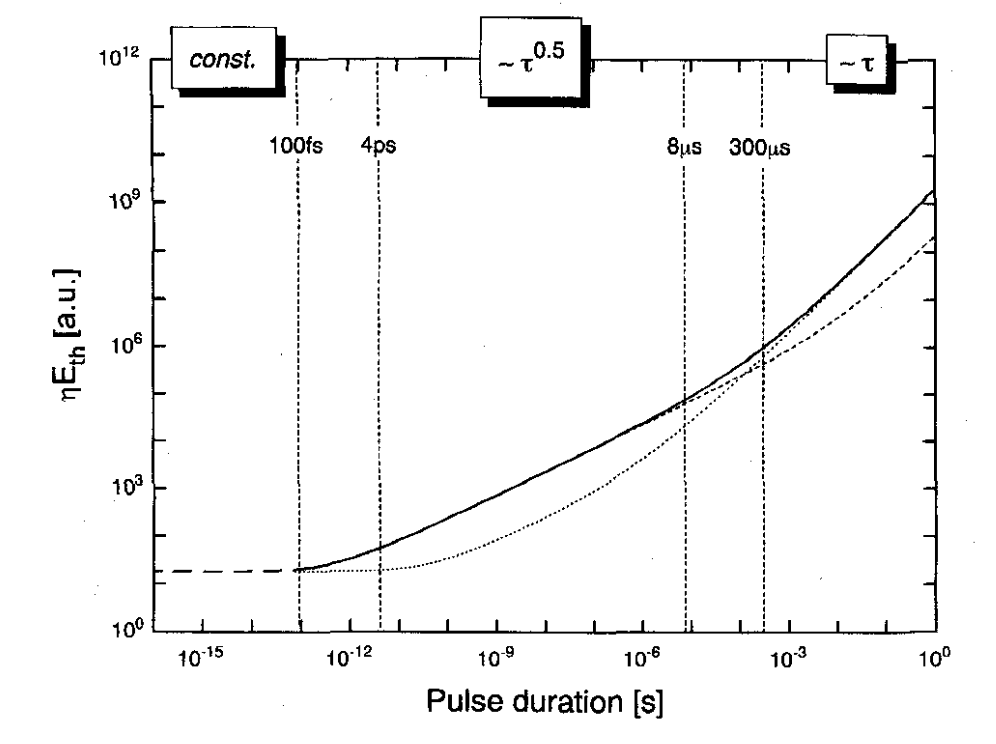
\includegraphics[width=\linewidth]{figures/Fig_loesel.png}
    \caption{Pulse duration dependence of breakdown threshold from Loesel \textit{et al.} \cite{loesel1996laserinduced-a8e}. The model includes collision ($\tau_c$) and diffusion ($\tau_d$) time constants; the solid line uses $\tau_c = 1$~fs and $\tau_d = 500$~ps, showing the characteristic square-root dependence in the nanosecond-to-picosecond regime.}
    \label{fig:fig_loesel}
\end{figure}

When both pulses operate near their threshold intensity levels, Eqs.~(\ref{eq:enhancement_fca}) and (\ref{eq:enhancement_tpa}) allow us to project the enhancement generated by GHz-burst-mode operation. However, operation at near ablation-threshold intensities is non-trivial since photoacoustic imaging applications are targeted for \textit{in vivo} imaging and biological tissue damage is governed by many different mechanisms, including photothermal damage and plasma-induced ablation \cite{Niemz2019}. Plasma-induced ablation is caused by high-intensity optical fields produced by ultrafast lasers ($\text{GW}/\text{cm}^{2}$). At these intensity levels, optical breakdown occurs as plasma starts to form due to avalanche ionization, resulting in rapid vaporization of the incident surface \cite{Niemz2019,boyd-2008}. Since the individual pulses interact with the tissue shorter than 1~$\mu$s, thermal diffusion is assumed to be negligible during individual pulse delivery \cite{Niemz2019}. However, since pulsed operation delivers many pulses to the interaction surface, heat accumulates, and thermal damage also starts to act as another limiting factor for the amount of energy delivered. For nonlinear imaging applications, the thermal damage threshold is determined around 2.5~mW for safe operation \cite{hopt-2001}.

\appendix

\section{Detailed enhancement derivations}

\subsection{Two-photon absorption enhancement}

Here we present the full algebraic derivation of the TPA enhancement factor stated in Eq.~(\ref{eq:enhancement_tpa}). From Eq.~(\ref{eq:heating_mpa}), the energy deposited per pulse is:
\begin{equation}
H = (\mu_a I + \beta I^2)\tau
\label{eq:energy_per_pulse}
\end{equation}
For a nanosecond pulse with intensity $I_0$ and duration $\tau_0$, the delivered total energy is $H_\text{ns} = (\mu_a I_0 + \beta I_0^2)\tau_0$. For a femtosecond burst with intensity $I_p$, pulse duration $\tau_p$, and $N$ pulses, the total energy is $H_\text{burst} = N(\mu_a I_p + \beta I_p^2)\tau_p$.

The enhancement factor is:
\begin{equation}
\varepsilon = \frac{H_\text{burst}}{H_\text{ns}} = \frac{N(\mu_a I_p + \beta I_p^2)\tau_p}{(\mu_a I_0 + \beta I_0^2)\tau_0}
\label{eq:enhancement_basic}
\end{equation}
Substituting Eq.~(\ref{eq:intensity_scaling}) into Eq.~(\ref{eq:enhancement_basic}) yields:
\begin{align}
\varepsilon &= N \times \frac{\mu_a I_0 \left(\frac{\tau_0}{\tau_p}\right)^\omega + \beta I_0^2 \left(\frac{\tau_0}{\tau_p}\right)^{2\omega}}{(\mu_a I_0 + \beta I_0^2)} \times \frac{\tau_p}{\tau_0} \nonumber \\[10pt]
&= N \times \frac{\mu_a\left(\frac{\tau_0}{\tau_p}\right)^{\omega-1} + \beta I_0\left(\frac{\tau_0}{\tau_p}\right)^{2\omega-1}}{(\mu_a + \beta I_0)}
\label{eq:enhancement_general}
\end{align}
When nonlinear absorption dominates ($\beta I_0 \gg \mu_a$), with $\omega = 0.75$, Eq.~(\ref{eq:enhancement_general}) simplifies to Eq.~(\ref{eq:enhancement_tpa}).

\subsection{Generalized $n$-photon enhancement}

The two-photon framework presented in the main text can be generalized to $n$-photon absorption by replacing $\beta I^2$ with $\beta_n I^n$, where $\beta_n$ is the $n$-photon absorption coefficient. When $n$-photon absorption dominates:
\begin{equation}
\varepsilon = \frac{N \beta_n I_p^n \tau_p}{\beta_n I_0^n \tau_0}
\label{eq:generalized_enhancement}
\end{equation}
Using the intensity scaling relation $I_p/I_0 = (\tau_0/\tau_p)^\omega$ and canceling $\beta_n$:
\begin{equation}
\varepsilon = N\left(\frac{\tau_0}{\tau_p}\right)^{n\omega-1}
\label{eq:gen_simp_enh}
\end{equation}
For $n = 2$ and $\omega = 0.75$, this recovers Eq.~(\ref{eq:enhancement_tpa}). For three-photon absorption ($n = 3$):
\begin{equation}
\varepsilon = N\left(\frac{\tau_0}{\tau_p}\right)^{1.25}
\label{eq:enhancement_3pa}
\end{equation}
Similarly, the FCA enhancement from Eq.~(\ref{eq:enhancement_fca}) generalizes to:
\begin{equation}
\varepsilon \sim N\left(\frac{\tau_0}{\tau_p}\right)^{n\omega-1} + C_n\,N(N-1)\left(\frac{\tau_0}{\tau_p}\right)^{(n+1)\omega-2}
\end{equation}
where $C_n = \sigma_\text{fc} I_0 \tau_0 / 2n\hbar\omega$.

\begin{backmatter}

\bmsection{Funding}
Content to be provided.

\bmsection{Acknowledgment}
Content to be provided.

\bmsection{Disclosures}
The authors declare no conflicts of interest.

\bmsection{Data Availability Statement}
Data underlying the results presented in this paper are not publicly available at this time but may be obtained from the authors upon reasonable request.

\end{backmatter}

%%%%%%%%%%%%%%%%%%%%%%% References %%%%%%%%%%%%%%%%%%%%%%%%%
\bibliography{references}

\end{document}
